
\begin{figure}
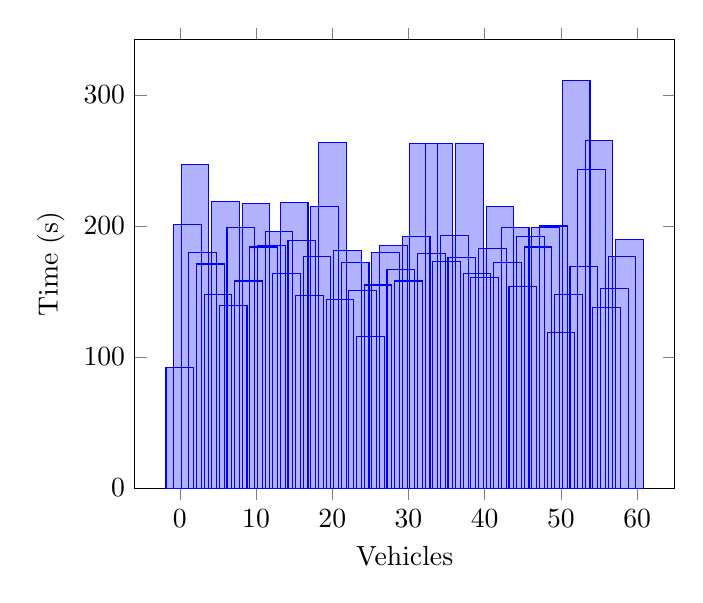
\begin{tikzpicture}
\begin{axis}[
legend style={anchor=west},
xlabel=Vehicles,
ylabel=Time (s),
ymin=0,
ybar,
]
\addplot coordinates {
(0, 92)
(1, 201)
(2, 247)
(3, 180)
(4, 171)
(5, 148)
(6, 219)
(7, 139)
(8, 199)
(9, 158)
(10, 217)
(11, 184)
(12, 185)
(13, 196)
(14, 164)
(15, 218)
(16, 189)
(17, 147)
(18, 177)
(19, 215)
(20, 264)
(21, 144)
(22, 181)
(23, 172)
(24, 151)
(25, 116)
(26, 155)
(27, 180)
(28, 185)
(29, 167)
(30, 158)
(31, 192)
(32, 263)
(33, 179)
(34, 263)
(35, 173)
(36, 193)
(37, 176)
(38, 263)
(39, 164)
(40, 161)
(41, 183)
(42, 215)
(43, 172)
(44, 199)
(45, 154)
(46, 192)
(47, 184)
(48, 199)
(49, 200)
(50, 119)
(51, 148)
(52, 311)
(53, 169)
(54, 243)
(55, 265)
(56, 138)
(57, 152)
(58, 177)
(59, 190)
};

\end{axis}
\end{tikzpicture}
\label{tik:100:3_V, 3_V.-60, 4_S, 5_S, 5_S.-30, 7_S, 7_S.-25, 11_S, 11_S.-50, 13_S, 15_N, 17_S, 17_S.-60, 18_S}
\caption{100 percent diving with GSC on route $3_V, 3_V.-60, 4_S, 5_S, 5_S.-30, 7_S, 7_S.-25, 11_S, 11_S.-50, 13_S, 15_N, 17_S, 17_S.-60, 18_S$}
\end{figure}
